\begin{figure}[H]
  \centering
  \hspace*{0cm}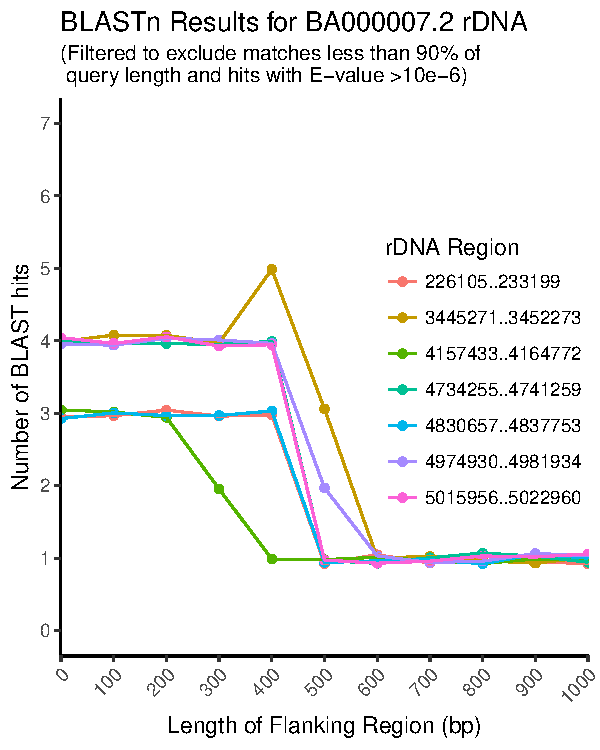
\includegraphics[width=.5\textwidth]{grouped_sakai_BLAST_results}
  \caption{BLASTn was used to perform \textit{in silico} DNA-DNA hybridization of all rDNA regions from \textit{E. coli Sakai} with variable flanking lengths. The number of hits is a proxy for occurrences in the genome; increasing the flanking length increases the specificity. (Points are jittered to aid visibility for overlapping values.)}
  \label{fig:blast}
\end{figure}
